\chapter{Análisis y Trazado de las Rectas de Carga}
\label{chap:rectas_de_carga}

El análisis gráfico mediante rectas de carga estática y dinámica permite visualizar las restricciones de excursión
de la etapa activa, verificando los márgenes de operación en zona lineal y garantizando que las señales de audio no
alcancen las regiones no lineales de corte o saturación.

\section{Recta de Carga Estática de Corriente Continua (CC)}

En corriente continua, los capacitores de acoplo se comportan como circuitos abiertos. En la topología colector común,
el colector se vincula directamente a $V_{CC}$ sin resistor de colector ($R_C = 0$), por lo que la resistencia total
de la malla de salida es exclusivamente la resistencia de emisor:
\begin{equation}
  R_{CC} = R_E = 1000\ohm = 1.0\kohm
  \label{eq:RCC_val}
\end{equation}

La ecuación de la malla de salida impone:
\begin{equation}
  V_{CC} = v_{CE} + i_C \cdot R_{CC} \implies i_C = -\frac{1}{R_E} \cdot v_{CE} + \frac{V_{CC}}{R_E}
  \label{eq:recta_cc}
\end{equation}

Los puntos notables de corte y saturación estáticos con los ejes coordenados son:
\begin{enumerate}
  \item Tensión de corte en continua ($i_C = 0$):
    \begin{equation}
      V_{CE,\mathrm{corte(CC)}} = V_{CC} = 5.00\V \implies (5.0\V,\ 0\mA)
    \end{equation}
  \item Corriente de saturación en continua ($v_{CE} = 0$):
    \begin{equation}
      I_{C,\mathrm{sat(CC)}} = \frac{V_{CC}}{R_E} = \frac{5.0\V}{1000\ohm} = 5.00\mA \implies (0\V,\ 5.0\mA)
    \end{equation}
\end{enumerate}

La pendiente de la recta estática es $m_{CC} = -1/R_E = -1.00 \times 10^{-3}\ohm^{-1}$.

\section{Recta de Carga Dinámica de Corriente Alterna (CA)}

A la frecuencia de trabajo de la señal ($1\kHz$), los capacitores de acoplo $C_1$ y $C_2$ presentan reactancias
despreciables, actuando como cortocircuitos. De este modo, la fuente $V_{CC}$ constituye masa dinámica y la carga
exterior $R_L$ queda conectada en paralelo con $R_E$ entre el emisor y masa. La resistencia de carga dinámica
vista desde el emisor resulta:
\begin{equation}
  R_{CA} = R_E \parallel R_L = \frac{R_E \cdot R_L}{R_E + R_L} = \frac{1000\ohm \cdot 10000\ohm}{1000\ohm + 10000\ohm} \approx 909.09\ohm
  \label{eq:RCA_val}
\end{equation}

La ley de variación dinámica alrededor del punto estático de reposo $Q(V_{CEQ} = 3.952\V,\ I_{CQ} = 1.043\mA)$ establece:
\begin{equation}
  i_C - I_{CQ} = -\frac{1}{R_{CA}} \cdot (v_{CE} - V_{CEQ})
\end{equation}
\begin{equation}
  i_C = -\frac{1}{R_{CA}} \cdot v_{CE} + \left(I_{CQ} + \frac{V_{CEQ}}{R_{CA}}\right)
  \label{eq:recta_ca}
\end{equation}

Los puntos de corte de la recta dinámica son:
\begin{enumerate}
  \item Tensión de corte dinámica ($i_C = 0$):
    \begin{equation}
      V_{CE,\mathrm{max(CA)}} = V_{CEQ} + I_{CQ} \cdot R_{CA} = 3.952\V + (1.043\mA \cdot 909.09\ohm) = 3.952\V + 0.948\V \approx 4.900\V
    \end{equation}
    correspondiente al punto coordenado $(4.90\V,\ 0\mA)$.
  \item Corriente de saturación dinámica ($v_{CE} = 0$):
    \begin{equation}
      I_{C,\mathrm{max(CA)}} = I_{CQ} + \frac{V_{CEQ}}{R_{CA}} = 1.043\mA + \frac{3.952\V}{909.09\ohm} = 1.043\mA + 4.347\mA \approx 5.390\mA
    \end{equation}
    correspondiente al punto coordenado $(0\V,\ 5.39\mA)$.
\end{enumerate}

La pendiente dinámica es $m_{CA} = -1/R_{CA} = -1.100 \times 10^{-3}\ohm^{-1}$, exhibiendo una inclinación levemente
mayor que la recta estática debido al efecto de carga de $R_L$.

\section{Gráfico de las Rectas de Carga y Márgenes de Excursión}

En la figura~\ref{fig:rectas_de_carga} se representa el diagrama conjunto de ambas rectas de carga en el plano
$i_C - v_{CE}$, destacando la posición del punto $Q$.

\begin{figure}[!ht]
  \centering
  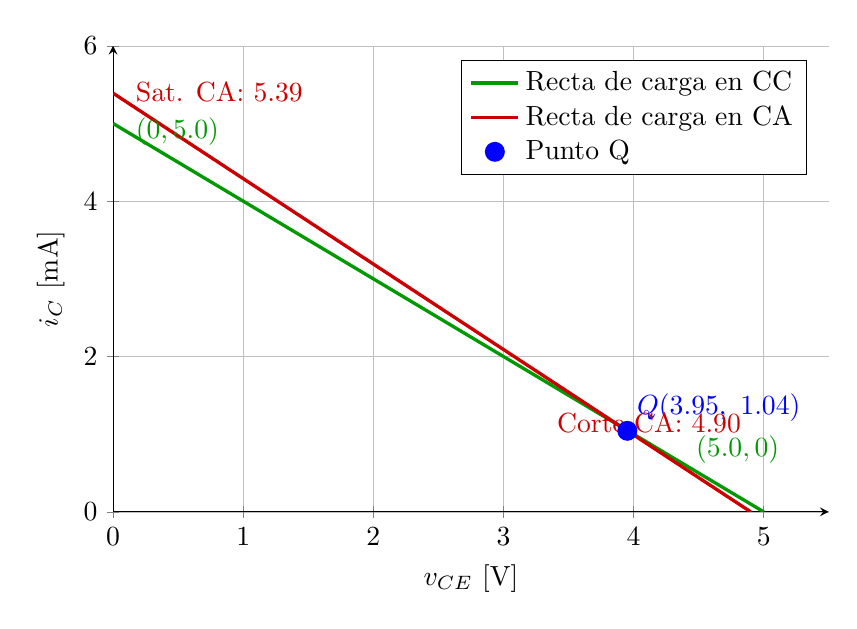
\begin{tikzpicture}
  \begin{axis}[
    width=0.88\textwidth,
    height=7.5cm,
    xlabel={$v_{CE}\ [\mathrm{V}]$},
    ylabel={$i_C\ [\mathrm{mA}]$},
    xmin=0, xmax=5.5,
    ymin=0, ymax=6.0,
    grid=both,
    grid style={line width=.1pt, draw=gray!30},
    major grid style={line width=.2pt,draw=gray!50},
    axis lines=left,
    legend pos=north east,
    legend cell align={left},
    every axis plot/.append style={very thick}
  ]
    % Recta de carga estatica (CC)
    \addplot[domain=0:5.0, color=green!60!black, samples=2] {5.0 - x};
    \addlegendentry{Recta de carga en CC }

    % Recta de carga dinamica (CA)
    \addplot[domain=0:4.90, color=red!80!black, samples=2] {1.043 + (3.952 - x)/0.90909};
    \addlegendentry{Recta de carga en CA }

    % Punto Q de reposo
    \addplot[only marks, mark=*, mark size=3pt, color=blue] coordinates {(3.952, 1.043)};
    \addlegendentry{Punto Q}

    % Anotaciones
    \node[above right, text=blue] at (axis cs:3.952, 1.043) {$Q(3.95\V,\ 1.04\mA)$};
    \node[above, text=green!60!black] at (axis cs:4.8, 0.5) {$(5.0\V, 0\mA)$};
    \node[right, text=green!60!black] at (axis cs:0.1, 4.9) {$(0\V, 5.0\mA)$};
    \node[above left, text=red!80!black] at (axis cs:4.9, 0.9) {Corte CA: $4.90\V$};
    \node[right, text=red!80!black] at (axis cs:0.1, 5.4) {Sat. CA: $5.39\mA$};
  \end{axis}
\end{tikzpicture}

  \caption{Rectas de carga estática (CC) y dinámica (CA) con indicación del punto $Q$ en el plano $i_C - v_{CE}$.}
  \label{fig:rectas_de_carga}
\end{figure}

A partir de la posición relativa del punto $Q$ se determinan los márgenes dinámicos admisibles:
\begin{itemize}
  \item Margen de excursión hacia la región de corte:
    \begin{equation}
      \Delta v_{CE,\mathrm{corte}} = V_{CE,\mathrm{max(CA)}} - V_{CEQ} = 4.900\V - 3.952\V = 0.948\V
    \end{equation}
  \item Margen de excursión hacia la región de saturación (considerando $V_{CE,\mathrm{sat}} \approx 0.20\V$):
    \begin{equation}
      \Delta v_{CE,\mathrm{sat}} = V_{CEQ} - V_{CE,\mathrm{sat}} = 3.952\V - 0.200\V = 3.752\V
    \end{equation}
\end{itemize}

El límite restrictivo viene impuesto por la excursión hacia el corte en el semiciclo negativo:
\begin{equation}
  \hat{v}_{o,\mathrm{max}} = \min(\Delta v_{CE,\mathrm{corte}},\ \Delta v_{CE,\mathrm{sat}}) = 0.948\V
\end{equation}
lo que determina una capacidad máxima de excursión pico a pico simétrica sin recorte de:
\begin{equation}
  v_{o,\mathrm{pp,max}} = 2 \cdot \hat{v}_{o,\mathrm{max}} \approx 1.896\Vpp \approx 1.90\Vpp
  \label{eq:vo_pp_max}
\end{equation}

Dado que la señal de entrada suministrada por el micrófono piezoeléctrico es de $200\mV_{\mathrm{rms}} \approx 0.57\Vpp$,
se comprueba que:
\begin{equation}
  v_{s,\mathrm{pp}} \approx 0.57\Vpp \ll 1.90\Vpp
\end{equation}
garantizando que la etapa amplificadora trabaja con amplio margen de seguridad dentro de su zona lineal activa,
asegurando una forma de onda libre de distorsiones armónicas y saturaciones.
